\chapter{Risultati}
In questo capitolo provvederemo ad analizzare i risultati dell'applicazione di GradCam alla CycleGAN secondo i metodi precedentemente descritti. Successivamente, descriveremo gli ulteriori sviluppi apportati alla rete e ne commenteremo i rispettivi risultati, confrontandoli tra loro grazie all'algoritmo FID.

\section{Introduzione}
Prima di vedere i risultati ottenuti descriviamo l'obiettivo della rete ed i parametri principali. La rete, come ampiamente spiegato, è una CycleGAN impiegata nella image-to-image translation. Nel nostro caso, il dataset scelto per addestrare e testare la rete è il dataset \emph{horse2zebra}. Il dataset è suddiviso in quattro parti: due per l'addestramento della rete, composte da 1334 immagini di cavalli e 1066 immagini di zebre, e due di test per la rete, composte da 120 cavalli e 139 zebre, per un totale di 2659 immagini.
\\Il numero di epoche necessarie a completare l'addestramento è 200, mentre il \emph{learning rate} della rete vale 0.0002 per le prime 100 epoche, successivamente andrà via via in diminuendo fino ad arrivare a 0.


\section{Addestramento base}
Prima di commentare i risultati ottenuti applicando GradCam alla rete, soffermiamoci sui risultati prodotti dalla rete non modificata. I risultati che ora andremo ad illustrare saranno quindi frutto dell'addestramento della CycleGAN proposta dal paper \cite{Zhu_2017_ICCV}. 
\subsection{Traduzione da cavalli a zebre}
Analizziamo i risultati ottenuti partendo dalla traduzione da cavalli a zebre. I risultati sono mediamente sufficienti, la rete in linea generale riesce a applicare le strisce che contraddistinguono le zebre sui cavalli, come vediamo in figura \ref{fig:Risultati Cycle GAN base (1)}.
\begin{figure}[H]
\begin{center}
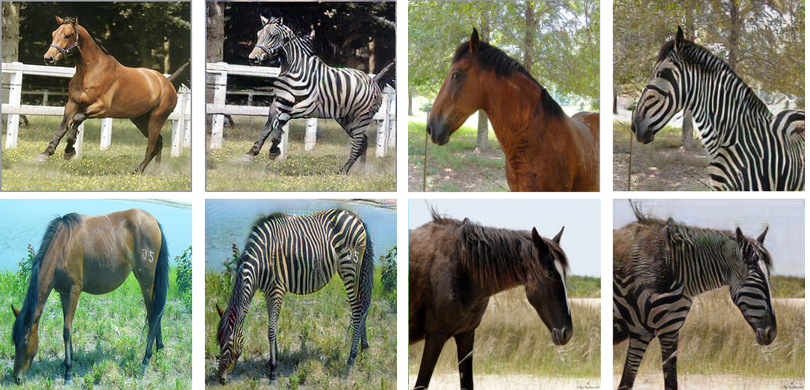
\includegraphics[width=1\columnwidth]{images/risultati cyclegan zebre.png}
\end{center}
\caption{Vediamo alcuni esempi di traduzione da cavallo a zebra dove la rete è riuscita a generare un'immagine accettabile.}
\label{fig:Risultati Cycle GAN base (1)}
\end{figure} 
Ovviamente la rete non è esente da difetti: in alcuni casi non riesce ad applicare uniformemente le strisce al manto del cavallo, rendendo evidente la falsità dell'immagine, oppure riconosce cavalli dove non ci sono, andando così a distorcere completamente l'immagine, come vediamo dagli esempi in figura \ref{fig:Risultati Errati Cycle GAN (1)} 

\begin{figure}[H]
\begin{center}
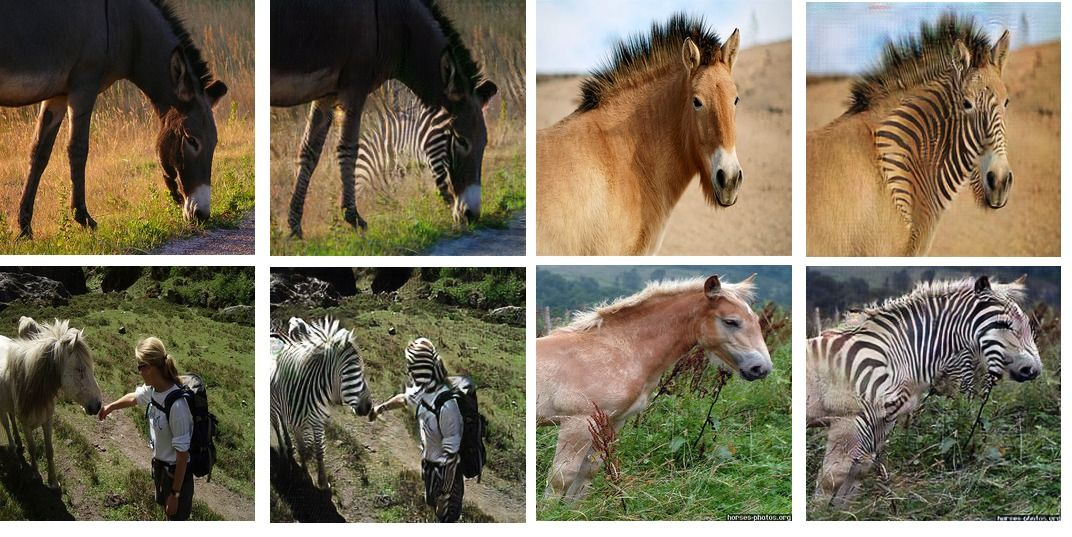
\includegraphics[width=1\columnwidth]{images/CycleGan zebre error.jpeg}
\end{center}
\caption{Vediamo come negli esempi di sinistra la rete non riesca a riconoscere il cavallo, mentre in quelli di destra la rete non riesca ad applicare le strisce in modo uniforme.}
\label{fig:Risultati Errati Cycle GAN (1)}
\end{figure} 

I risultati migliori sono quelli ottenuti da immagini in cui il cavallo è ben riconoscibile in foto e non è distante. La rete, inoltre, ha difficoltà a riconoscere la sagoma del cavallo quando nella foto sono presenti più cavalli, soprattutto se sovrapposti in prospettiva. L'algoritmo di FID applicato alle immagini delle zebre generate dalla rete, rispetto a tutte le immagini delle zebre del dataset, restituisce come risultato 33.66.
\subsection{Traduzione da zebre a cavalli}
Valutiamo ora la traduzione contraria, da zebre a cavalli. In questo caso, notiamo come la rete abbia più difficoltà nella generazione delle immagini, come vediamo in figura \ref{fig:Risultati Horse Cycle GAN (1)}. E' infatti difficile trovare tra i risultati immagini pienamente soddisfacenti, che mettano in difficoltà anche l'occhio umano, cosa che invece, nel caso precedente, accadeva con più frequenza.
\begin{figure}[H]
\begin{center}
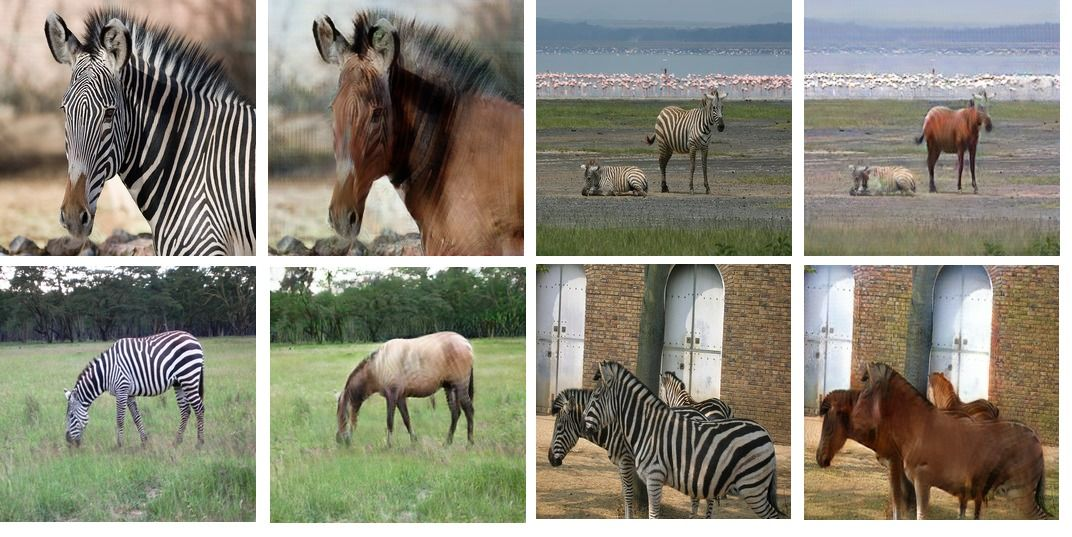
\includegraphics[width=1\columnwidth]{images/CycleGan horse (1).jpeg} 
\end{center}
\caption{Alcuni dei migliori risultati della traduzione da zebre a cavalli, vediamo come rimangano le strisce che la rete prova ad eliminare.}
\label{fig:Risultati Horse Cycle GAN (1)}
\end{figure} 
In questo caso l'algoritmo di FID, applicato rispetto a tutte le immagini dei cavalli presenti nel dataset, restituisce come risultato 64.57.

\section{Addestramento con trasferimento dell'attenzione}
Vediamo ora i risultati ottenuti dalla rete modificata utilizzando GradCam per generare la Loss di consistenza dell'attenzione. Sono stati effettuati più addestramenti con questa modalità, cambiando i parametri su cui ricavare l'attenzione, come vedremo successivamente. In questa sezione ci soffermeremo sui risultati ottenuti applicando il trasferimento dell'attenzione sull'ultimo blocco residuo. In questo caso, i risultati sono notevolmente migliorati nella traduzione da cavalli a zebre e hanno avuto un leggero miglioramento anche nella traduzione opposta.
\subsection{Traduzione da cavalli a zebre}
Come detto, si è migliorata l'efficienza della rete nella traduzione da cavalli a zebre. Infatti, i risultati mostrano una maggiore precisione nel riconoscimento del cavallo a cui applicare le strisce e una maggiore capacità di uniformare i cambiamenti. Come vediamo in figura \ref{fig:Risultati Zebre CycleGan + GradCam}, la rete genera, infatti, risultati migliori e più verosimili.
\\Ovviamente, anche in questo caso la rete non è perfetta, sono ancora presenti alcuni problemi nel riconoscimento dei cavalli in determinate foto, come ad esempio quelle ritraenti più cavalli distanti dall'obiettivo.

\begin{figure}[H]
\begin{center}
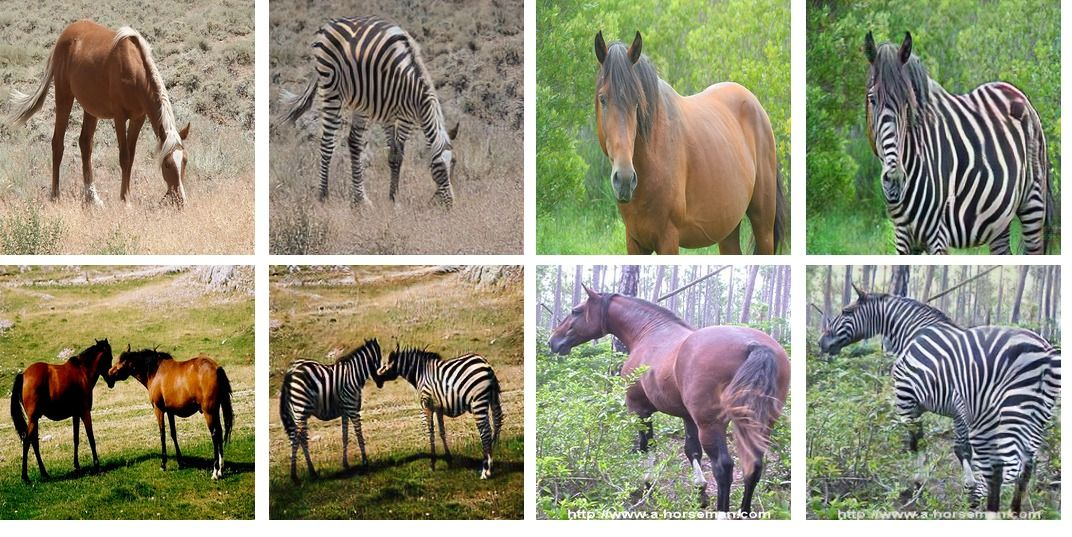
\includegraphics[width=1\columnwidth]{images/CycleGan + GradCam zebre.jpeg} 
\end{center}
\caption{Alcuni dei migliori risultati della traduzione da cavalli a zebre con trasferimento dell'attenzione, vediamo come le strisce siano più marcate ed uniformi.}
\label{fig:Risultati Zebre CycleGan + GradCam}
\end{figure} 

A sostegno di quanto affermato possiamo utilizzare l'algoritmo di FID ottenendo un risultato di 27.9.

\subsection{Traduzione da zebre a cavalli}
Come affermato precedentemente, in questo caso il miglioramento è minimo. Infatti, la rete fa ancora fatica ad eliminare uniformemente le strisce bianche e nere delle zebre, come vediamo dalla figura \ref{fig:Risultati cavalli GradCam}. I risultati sono molto simili ai precedenti, lo dimostra anche il risultato del FID, pari a 61.5, ancora molto elevato.
\begin{figure}[H]
\begin{center}
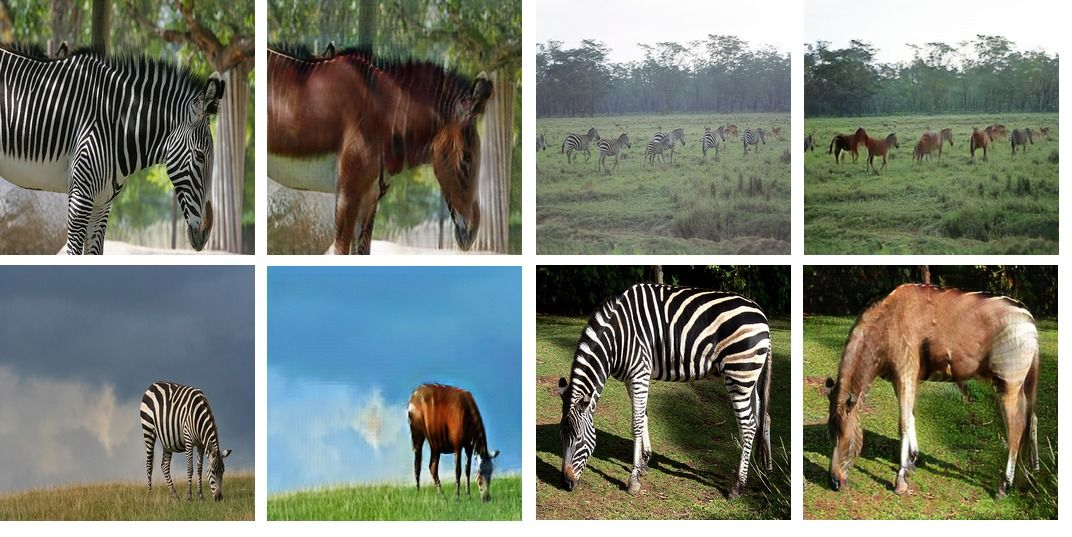
\includegraphics[width=1\columnwidth]{images/image (2).jpeg} 
\end{center}
\caption{Alcuni dei migliori risultati della traduzione da zebre a cavalli, vediamo come, anche in questo caso, rimangano le strisce che la rete prova ad eliminare.}
\label{fig:Risultati cavalli GradCam}
\end{figure} 

\section{Confronto tra le due reti}
Abbiamo dunque visto come la rete venga migliorata applicando il trasferimento dell'attenzione. Ora possiamo andare nel dettaglio e, aiutandoci tramite esempi generati da entrambe le reti, confrontare i risultati.
\\\emph{Per comodità le reti verranno da qui in poi indicate come rete \emph{standard} e rete \emph{GradCam}}
\\Nella sezione precedente, avevamo indicato tra i problemi della rete \emph{standard} la difficoltà nell'applicare in maniera uniforme le strisce bianche e nere ai cavalli; questo problema, come vediamo in figura \ref{fig:Confronto GradCam e noGradCam}, viene perfettamente risolto dalla rete \emph{GradCam}. Inoltre, le immagini generate dalla rete \emph{GradCam} hanno mediamente una qualità migliore rispetto alle altre. Questo lo si nota andando ad analizzare lo sfondo delle immagini generate: nel caso \emph{standard}, molto spesso, esso risultava essere corrotto, oppure perdeva colore, risultando la maggior parte delle volte più scuro e opaco. Nel caso della rete \emph{GradCam}, invece, lo sfondo risente meno di questi peggioramenti, come notiamo dal colore del cielo della prima immagine della figura \ref{fig:Confronto GradCam e noGradCam}, e ciò porta ad una migliore qualità nel complesso. La rete \emph{GradCam} è inoltre in grado di riconoscere meglio i cavalli: infatti alcuni di essi, specie quelli dal manto completamente nero, mettevano in seria difficoltà la rete \emph{standard}, mentre la rete \emph{GradCam}, seppur non ancora in maniera ottimale, riesce a portare buoni risultati anche su questa tipologia di immagini.
Un ulteriore miglioramento che salta all'occhio risiede nel colore del manto delle zebre generate dalla rete \emph{GradCam}: molto spesso infatti, anche nelle migliori immagini generate dalla rete \emph{standard}, il manto presentava sfumature scure, tendenti al marrone, dovute al colore del cavallo originale. Nelle immagini prodotte dalla rete \emph{GradCam}, invece, queste sfumature si sono, nella maggior parte delle immagini, azzerate.



\begin{figure}[H]
\begin{center}
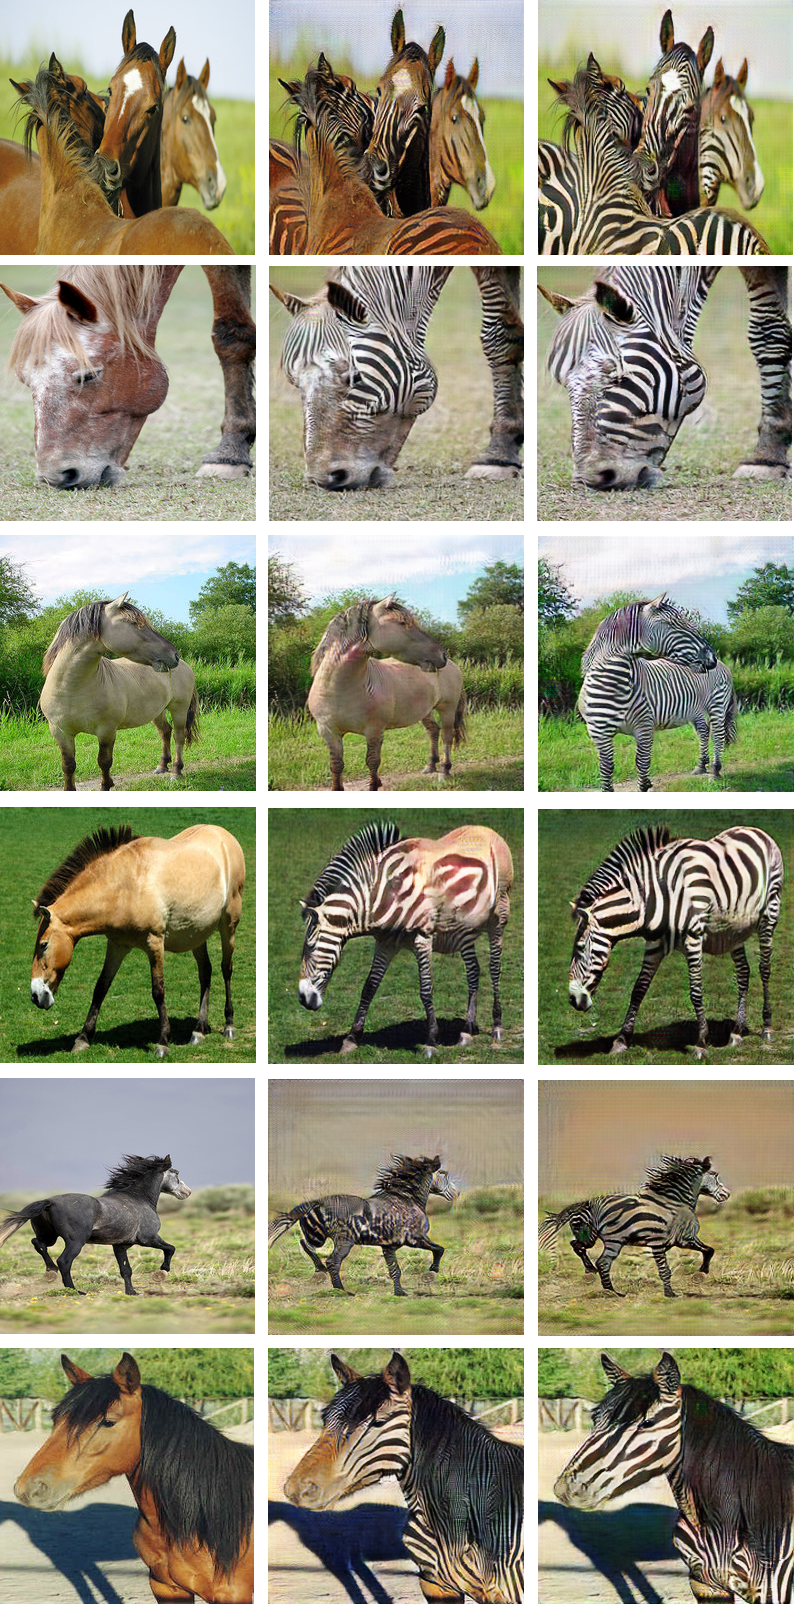
\includegraphics[width=0.6\columnwidth]{images/merge zebre.png}
\end{center}
\caption{In foto il confronto tra immagine reale, immagine generata senza GradCam e immagine generata dalla rete con GradCam.}
\label{fig:Confronto GradCam e noGradCam}
\end{figure}  
Un discorso simile lo si può fare anche trattando la traduzione da zebre a cavalli: infatti, seppur i risultati siano ancora lontani dalla realtà, possiamo notare alcuni miglioramenti. Come vediamo in figura \ref{fig:Confronto GradCam e noGradCam cavalli}, la rete \emph{GradCam} si dimostra migliore nell'eliminazione delle strisce bianche e nere, specie in quelle immagini che ritraggono le zebre in primo piano. 
\\Nonostante questi miglioramenti, rimane però il problema principale che caratterizzava la rete \emph{standard}: non si riescono ad eliminare perfettamente le strisce delle zebre. Entrambe le reti, infatti, non mostrano particolare difficoltà nel differenziare l'animale dallo sfondo, cosa che accade nella traduzione opposta, ma hanno elevata difficoltà nell'eliminazione delle strisce bianche e nere, tant'è che la maggior parte dei risultati presenta ancora strascichi delle strisce, come vediamo dalla figura \ref{fig:Confronto GradCam e noGradCam cavalli}.


\begin{figure}[H]
\begin{center}
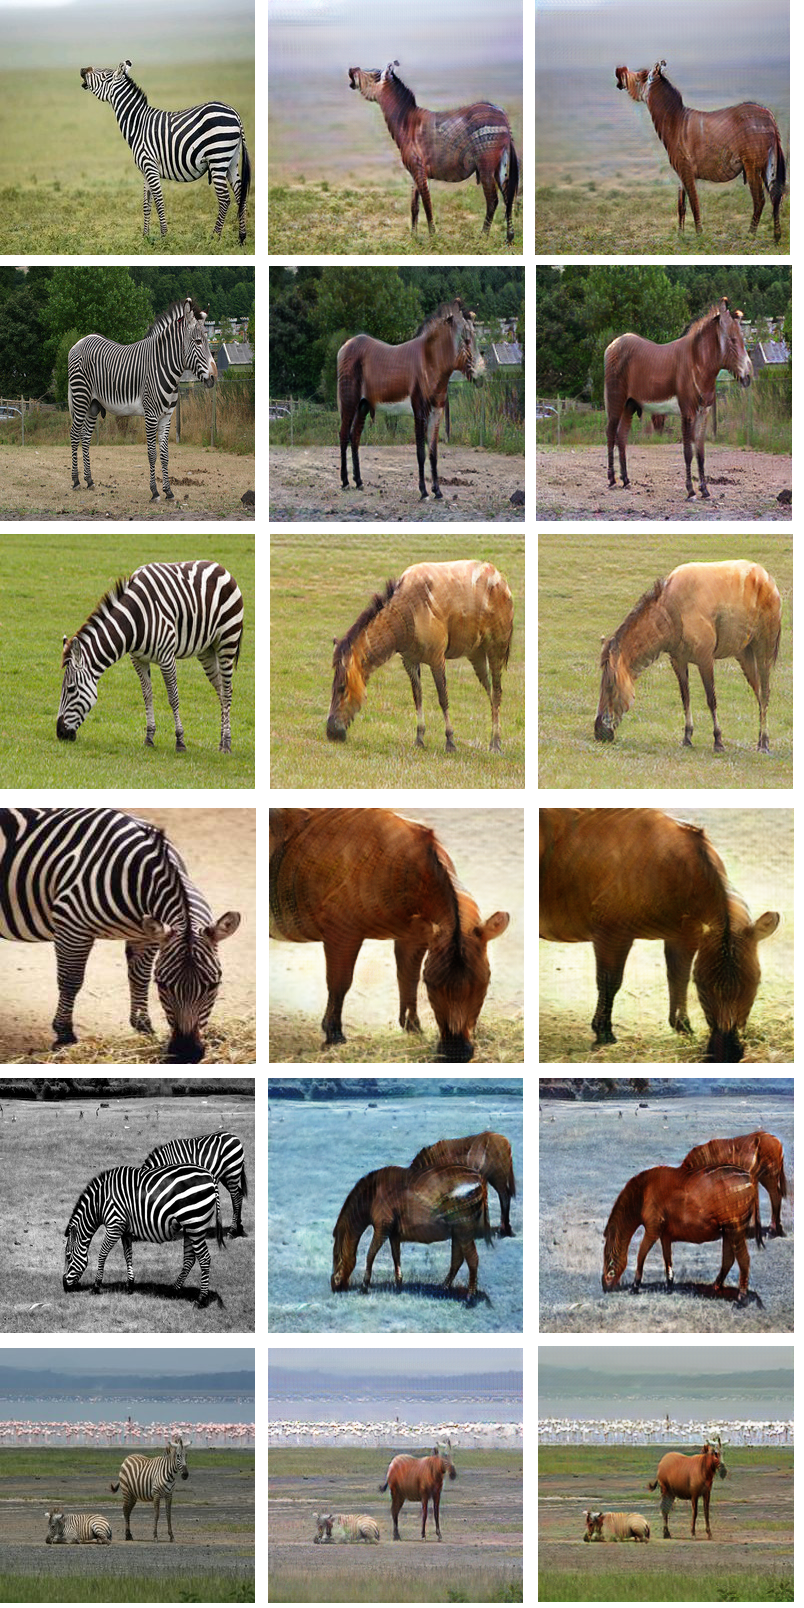
\includegraphics[width=0.6\columnwidth]{images/merge.png}
\end{center}
\caption{In foto il confronto tra immagine reale, immagine generata senza GradCam e immagine generata dalla rete con GradCam.}
\label{fig:Confronto GradCam e noGradCam cavalli}
\end{figure}  

\section{Ulteriori sviluppi per la rete}
Dopo aver commentato i risultati ottenuti sfruttando GradCam sull'ultimo blocco residuo ed averli confrontati con i risultati della rete \emph{standard}, possiamo ora analizzare le ulteriori modifiche che abbiamo apportato alla rete. Infatti, al fine di migliorare i risultati ottenuti, abbiamo provato a modificare alcuni parametri della rete, sempre utilizzando l'algoritmo GradCam. Prima di entrare nel dettaglio, è bene specificare che tra tutte le reti provate, quella migliore, basandoci sul risultato dell'algoritmo FID, rimane la rete \emph{GradCam}, come vediamo dalla tabella \ref{tab:Fid Table}.
\\Le modifiche apportate alla rete sono state le seguenti:
\begin{itemize}
\item Utilizzo di un coefficiente pari a 0.1 per la Loss di consistenza dell'attenzione;
\item Utilizzo di GradCam solo nella traduzione \emph{primaria}, quindi solo da dal dominio $A$ al dominio $B$;
\item Utilizzo di GradCam attraverso un \emph{detach} sulle immagini fake generate per il calcolo della Loss;
\item Utilizzo di GradCam su quattro blocchi residui.
\end{itemize}



\begin{center}
\begin{tabular}{ | c | c | c | }
\hline
\textbf{Rete}          & \textbf{FID Zebre}        &   \textbf{FID Cavalli}    \\
\hline
\emph{standard}          & 33.66     & 64.57  \\ \hline
\emph{GradCam}           & 27.94     & 61.54  \\ \hline
\emph{GradCamWithCoeff}  & 31.90     & 66.01  \\ \hline
\emph{GradCamA2B}        & 30.60     & 65.32  \\ \hline
\emph{GradCamWithDetach} & 32.74     & 62.71  \\ \hline
\emph{GradCamFourLayers}   & 33.18     & 61.77  \\ \hline
\end{tabular}
\captionof{table}{Comparazioni tra i valori dei FID delle varie architetture utilizzate.}
\label{tab:Fid Table}
\end{center}

Andando più nel dettaglio vediamo perchè abbiamo provato queste modifiche alla rete.
\\Per quanto riguarda il coefficiente applicato alla Loss di consistenza dell'attenzione, abbiamo ragionato sul fatto che, senza questo coefficiente, la Loss sarebbe potuta essere troppo elevata rispetto alle altre presenti all'interno della rete, e, per questo motivo, avrebbe potuto sbilanciare il calcolo più in suo favore, riducendo i contributi delle altre Loss.
\\Il ragionamento che ci ha spinti, invece, ad utilizzare GradCam solo per la traduzione da $A$ a $B$ invece è dovuto al fatto di voler provare ad utilizzare il trasferimento dell'attenzione solo per la traduzione da cavalli a zebre, in quanto è in questa traduzione che si riscontrano i risultati migliori.
\\L'utilizzo del \emph{detach} sulle immagini fake durante il calcolo della Loss, di cui vediamo il codice:
\begin{minted}[bgcolor= lightGray]{Python}
self.att_lossA2B = self.MSE_LOSS(self.cam_fake_B.detach(),
                             self.cam_rec_A)
self.att_lossB2A = self.MSE_LOSS(self.cam_fake_A.detach(),
                             self.cam_rec_B)
\end{minted}
è stato fatto perchè senza di esso sono entrambe le attenzioni che tendono ad un'attenzione comune, sia quella dell'immagine reale che quella dell'immagine fake. Idealmente, però, sarebbe solo l'attenzione dell'immagine fake a doversi adattare a quella dell'immagine reale, ed è proprio a questo che serve il \emph{detach} posto prima del calcolo della Loss.
\\Infine, l'utilizzo di GradCam su quattro blocchi residui, anzichè solo sull'ultimo, è stato effettuato per provare a migliorare la consistenza dell'attenzione. I layer scelti (10,14,15,18), infatti, mostravano i risultati migliori nella generazione delle attenzioni.
Concludiamo questa sezione andando a vedere i risultati generati dalle varie reti sulle stesse immagini. Come vediamo dalle figure \ref{fig:Confronto tra tutte le reti zebre} \ref{fig:Confronto tra tutte le reti cavalli}, la rete \emph{GradCam} si conferma la migliore.


\begin{figure}[H]
\begin{center}
\includegraphics[width=1\columnwidth]{images/allOrdine.png}
\end{center}
\caption{In foto il confronto tra le immagini generate dalle reti, ordinate decrescentemente da sinistra a destra secondo il risultato dell'algoritmo di FID.}
\label{fig:Confronto tra tutte le reti zebre}
\end{figure}  

\begin{figure}[H]
\begin{center}
\includegraphics[width=1\columnwidth]{images/All Cavalli.png}
\end{center}
\caption{In foto il confronto tra le immagini generate dalle reti, ordinate decrescentemente da sinistra a destra secondo il risultato dell'algoritmo di FID.}
\label{fig:Confronto tra tutte le reti cavalli}
\end{figure}  